\documentclass{article}
\usepackage{amsmath,amssymb,graphicx,hyperref,booktabs,float,subcaption}
\usepackage[margin=1in]{geometry}

\begin{document}

\begin{titlepage}
    \centering
    \vspace*{2.5cm}
    
    {\LARGE \textbf{DS 3000: Introduction to Machine Learning}}\\[0.5cm]
    {\Large \textbf{Canadian Households Coursework}}\\[1.5cm]
    
    {\Huge \textbf{Analysis of Canadian Household Demographics \\[0.3cm] and Spending Patterns}}\\[2cm]

    {\large \textbf{Group 9}}\\[0.8cm]
    \begin{tabular}{rl}
        Namra Patel & \hspace{1cm} npate334 \\
        Moksh Trehan & \hspace{1cm} mtrehan2 \\
        Daehan Lee & \hspace{1cm} dlee739 \\
        Sepehr Seghatoleslami & \hspace{1cm} sseghato \\
    \end{tabular}
    
    \vfill
    {\large \textbf{Word Count: 2337}}\\[1.5cm]    
    {\large April 2025}
\end{titlepage}


\tableofcontents
\newpage	

\section{Executive Summary}

This project analyzes Canadian household data to identify patterns in demographic and economic behavior using clustering and dimensionality reduction, followed by predictive modeling of insurance and pension spending.

\subsection*{1. Clustering and Dimensionality Reduction}

We began with data cleaning, removing 47 variables closely tied to the target to avoid leakage. Given the mismatch between metadata and dataset, variables not found were logged and the rest removed. Outliers were handled conservatively using IQR-based winsorization, chosen for its robustness in skewed data.

To uncover household clusters, we applied K-Means clustering. Elbow and Silhouette methods agreed that the optimal cluster number was likely 2 or 3, but both indicated weak clustering structure. We proceeded with $K = 3$ for further analysis.

PCA was used to reduce dimensionality. We compared results on scaled and unscaled data, choosing the scaled version for interpretability despite higher raw variance in the unscaled results. PC1 (67.9\% variance) captured economic activity and household size; PC2 reflected immigrant presence versus native-established populations; PC3 related to household structure and living arrangements.

Cluster interpretation yielded:
\begin{itemize}
    \item \textbf{Cluster 0:} Affluent immigrant families with high spending and traditional structures.
    \item \textbf{Cluster 1:} Low-spending, high-immigration, small households.
    \item \textbf{Cluster 2:} Native-born, mid-spending, non-traditional households.
\end{itemize}

UMAP was applied for further visualization using tuned hyperparameters. Euclidean distance with \texttt{n\_neighbors=40} and \texttt{min\_dist=1} showed best separation. UMAP produced clearer cluster boundaries than PCA, particularly highlighting differences in household composition and immigrant status.

\subsection*{2. Regression Modeling for Insurance \& Pension Spending}

The target variable was defined as the proportion of income spent on personal insurance and pensions. We excluded related features to prevent leakage and cleaned the dataset through imputation, low-variance feature removal, and IQR-based winsorization. The resulting features were standardized and categorical variables one-hot encoded.

Two models were developed:
\begin{itemize}
    \item \textbf{Elastic Net Regression} achieved an $R^2$ of 0.8040 (95\% CI: [0.8020, 0.8058]) with MSE of 0.1966. Top predictors included employment/unemployment rates, median age, and miscellaneous household spending. These captured macroeconomic and demographic signals, showing strong but linear effects.
    \item \textbf{XGBoost Regression} significantly outperformed Elastic Net, with $R^2$ of 0.9114 (95\% CI: [0.9105, 0.9123]) and MSE of 0.0888. It captured non-linear patterns missed by Elastic Net, including threshold effects for housekeeper count and gift contributions.
\end{itemize}

SHAP analysis on the XGBoost model confirmed the importance of variables such as number of housekeepers, secondary mortgage, gift spending, median maintainer age, and childcare expenses. These insights emphasized the non-linear and interactive nature of the problem, supporting the use of XGBoost over linear models.

\subsection*{Recommendations}
\begin{itemize}
    \item Deploy XGBoost with SHAP-based monitoring for explainability.
    \item Segment users by key drivers (e.g., maintainer age, household support).
    \item Expand the dataset with behavioral variables for more granular targeting.
    \item Use A/B testing to measure impact of model-driven interventions.
\end{itemize}

\section{Clustering and Dimensionality Reduction}
In this section we outline the process and results of applying the K-Means Clustering algorithm, and the Principal Component Analysis (PCA) and the Uniform Manifold Approximation and Projection (UMAP) dimensionality reduction techniques to learn if there are segments or axes of grouping in our data that allow us to uncover meaningful patterns or characteristics and guide subsequent predictive modeling.

\subsection{Data Preprocessing}

To prepare the data for clustering and dimensionality reduction, we first merged the DemoStats and HouseholdSpend datasets using Dissemination Area (DA) identifiers, then dropped the identifier columns as they offered no predictive value.

We addressed missingness by identifying variables, mostly median age-related, with over 10\% null values. Despite this, they showed meaningful correlation with the target variable, so we retained them and imputed missing values using the column medians.

To avoid information leakage into unsupervised learning, we removed 47 variables tied to our regression target, including those containing terms like ‘income’, ‘insurance’, ‘pension’, ‘retirement’, and ‘tax’. This prevented clustering from being influenced by features directly related to the dependent variable in the regression.

Given the skewed nature of our dataset, we handled outliers using IQR-based winsorization, capping extreme values at 1.5× the interquartile range. This method was preferred over z-score trimming, which would have reinforced distribution skewness.

Finally, we applied z-score normalization to all numeric features. As K-Means and PCA are scale-sensitive, standardization ensures fair comparison across features.

\subsection{K-Means Clustering}

Due to the dataset’s size, we applied the Elbow and Silhouette methods on a 10\% sample to estimate an appropriate number of clusters for K-Means while minimizing compute overhead.

The Elbow method (Figure~\ref{fig:elbow}) shows a bend at $k=4$, indicating diminishing returns in distortion reduction beyond this point.

\begin{figure}[H]
    \centering
    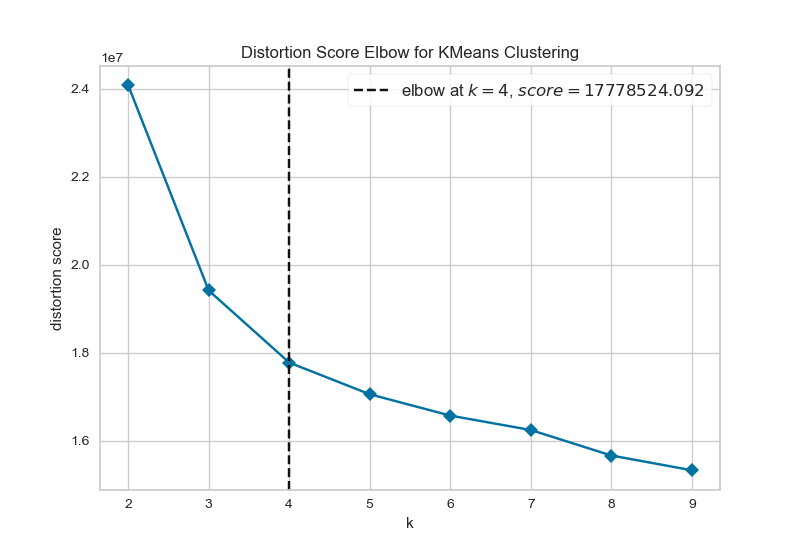
\includegraphics[width=0.7\textwidth]{figures/elbow_plot.png}
    \caption{Distortion Score Elbow for KMeans Clustering}
    \label{fig:elbow}
\end{figure}

Silhouette plots for $k=2$, $k=3$, and $k=4$ (Figures~\ref{fig:silhouette_k2}–\ref{fig:silhouette_k4}) illustrate a trade-off between cohesion and interpretability. $k=2$ (Figure~\ref{fig:silhouette_k2}) yields the highest average score but produces overly broad clusters. $k=3$ (Figure~\ref{fig:silhouette_k3}) shows clearer separation with moderate cohesion. At $k=4$ (Figure~\ref{fig:silhouette_k4}), cohesion declines further with increased overlap.

\begin{figure}[H]
    \centering
    \begin{minipage}{0.50\textwidth}
        \centering
        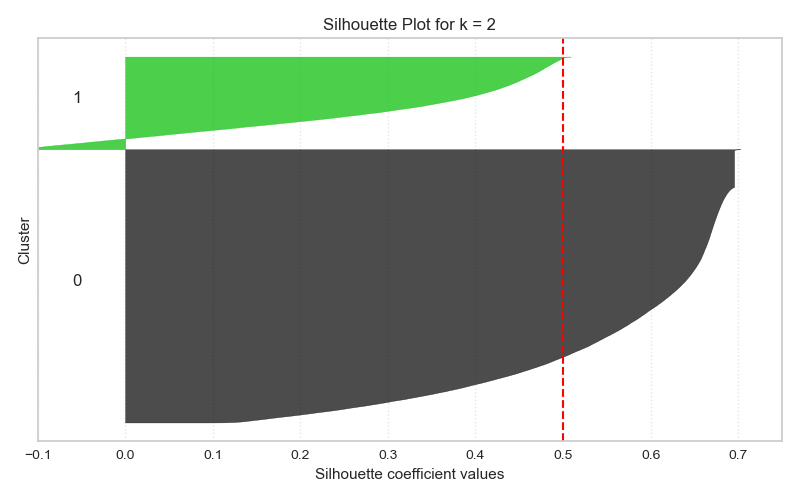
\includegraphics[width=\linewidth]{figures/silhouette_k2.png}
        \caption{Silhouette Plot for $k=2$}
        \label{fig:silhouette_k2}
    \end{minipage}\hfill
    \begin{minipage}{0.50\textwidth}
        \centering
        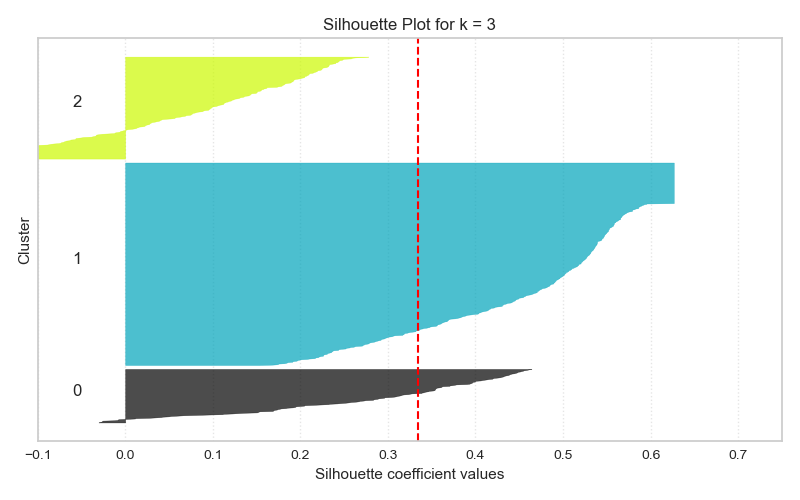
\includegraphics[width=\linewidth]{figures/silhouette_k3.png}
        \caption{Silhouette Plot for $k=3$}
        \label{fig:silhouette_k3}
    \end{minipage}
\end{figure}

\begin{figure}[H]
    \centering
    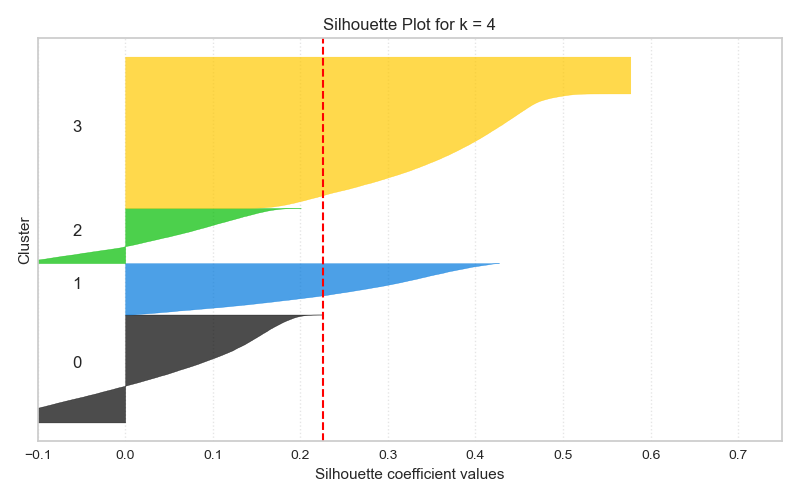
\includegraphics[width=0.50\textwidth]{figures/silhouette_k4.png}
    \caption{Silhouette Plot for $k=4$}
    \label{fig:silhouette_k4}
\end{figure}


The Silhouette plot for $k=5$ (Figure~\ref{fig:silhouette_k5}) and average Silhouette scores across $k=2$ to $k=5$ (Figure~\ref{fig:silhouette_scores}) are included in the appendix.

Given the interpretability and moderate separation at $k=3$, we selected it as the final number of clusters. These labels were retained for dimensionality reduction and further analysis.


\subsection{Principal Component Analysis}

To explore latent structure in the data, we applied Principal Component Analysis (PCA), a linear dimensionality reduction technique. We compared results on both unscaled and standardized data. Although PCA on unscaled data yielded a first component that explains 98.8\% of the variance, this result was driven largely by the presence of features with larger numeric scales. In contrast, the scaled version, where all variables are z-score normalized, produced a more balanced set of principal components, with the first three PCs explaining 67.9\%, 3.7\%, and 3.0\% of the variance, respectively. Therefore, all PCA analyses moving forward are based on the scaled data.

Figure~\ref{fig:pca3d} illustrates 3D scatterplots of the first three principal components for both the unscaled and scaled data, coloured by the K-Means cluster labels ($k=3$). The scaled data plot reveals broad, loosely separated regions aligned with the cluster assignments, though some overlap remains, suggesting that the clustering structure is not sharply defined but does capture some underlying gradients in the data.

\begin{figure}[H]
    \centering
    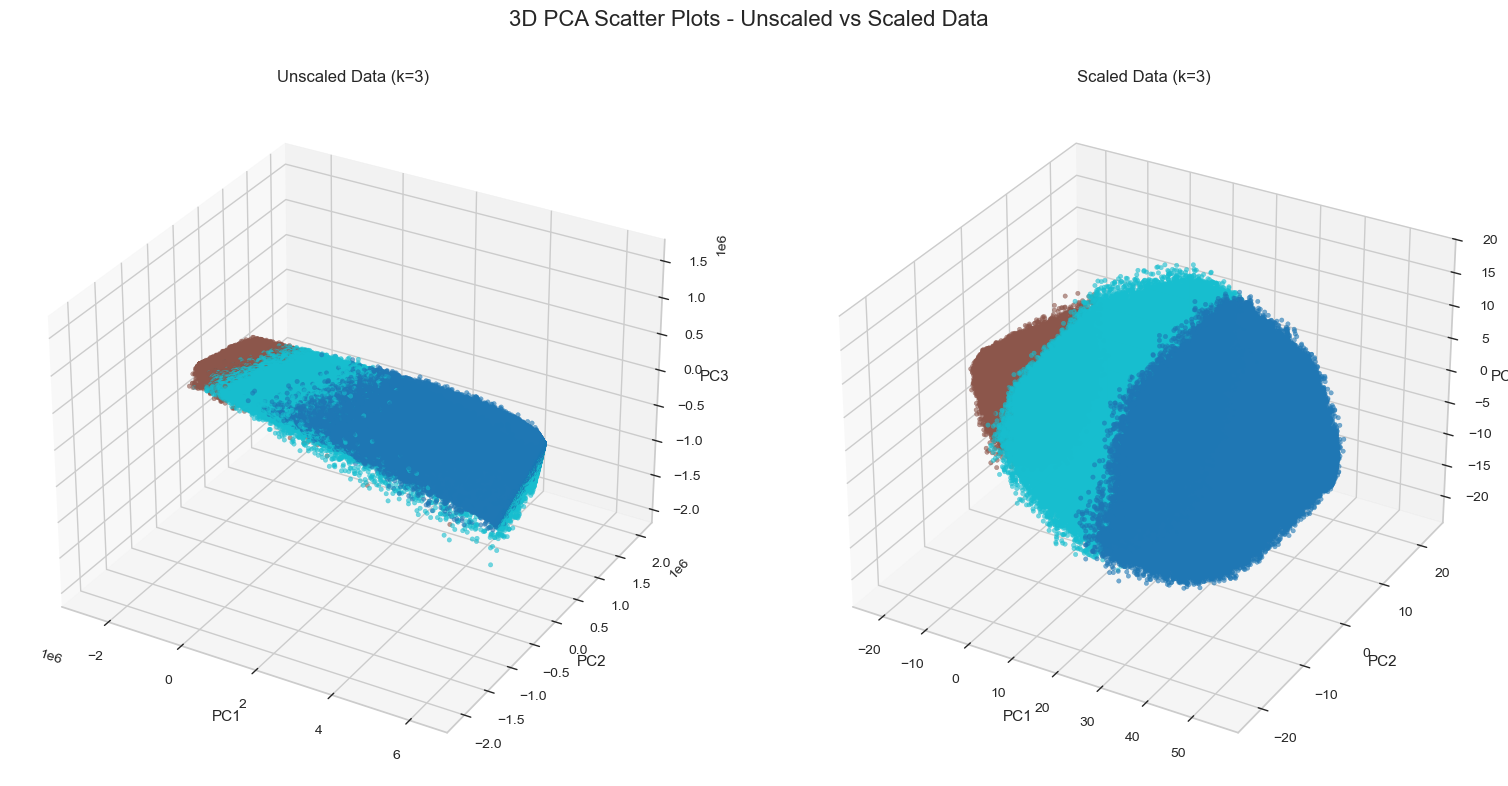
\includegraphics[width=0.8\textwidth]{figures/pca3d_scaled_vs_unscaled.png}
    \caption{3D PCA Scatter Plots Comparing Unscaled (Left) vs. Scaled (Right) Data}
    \label{fig:pca3d}
\end{figure}

We calculated the top five positive and negative contributors to each of the first three principal components and grouped them by variable category for interpretability. The detailed variable-level contributions are presented in Appendix Tables~\ref{tab:pc1_pos}--\ref{tab:pc3_neg}.

\paragraph{PC1: Economic Activity and Household Presence.}  
PC1 appears to capture a dimension tied to household economic activity and consumer behavior. The dominant contribution from the \textit{Consumption} category (Figure~\ref{fig:pc1}) suggests that higher PC1 scores are associated with greater household spending. This is supported by additional contributions from population-related categories like \textit{Total Household Population by Age}, indicating these are also demographically dense areas. Contributions from \textit{Household Population 15+ by Industry} further reinforce the interpretation that PC1 reflects regions with economically active residents and a strong consumer presence.

\begin{figure}[H]
    \centering
    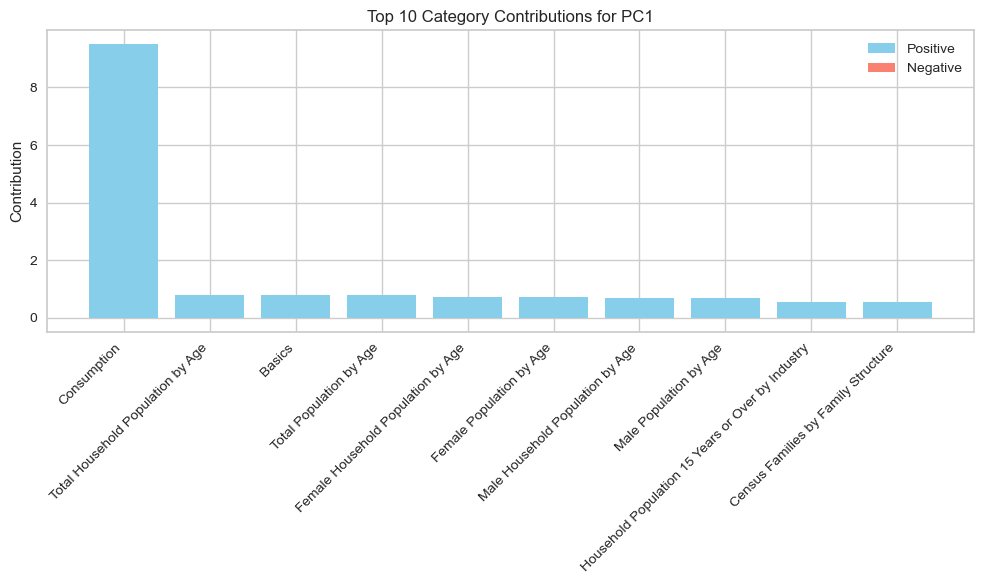
\includegraphics[width=0.8\textwidth]{figures/pc1_contribs.png}
    \caption{Top Contributing Categories to PC1}
    \label{fig:pc1}
\end{figure}

\paragraph{PC2: Immigrant Presence vs. Established Households.}  
PC2 differentiates areas with high immigrant presence from those with more established populations (Figure~\ref{fig:pc2}). While \textit{Consumption} remains a positive factor, the strongest negative contributions come from immigration-related categories such as \textit{Total Immigrants and Place of Birth}, \textit{Period of Immigration}, and \textit{Age at Immigration}. High PC2 scores likely reflect long-established, non-immigrant populations with moderate spending, while lower scores correspond to recent immigrant-dense areas with distinct demographic structures.

\begin{figure}[H]
    \centering
    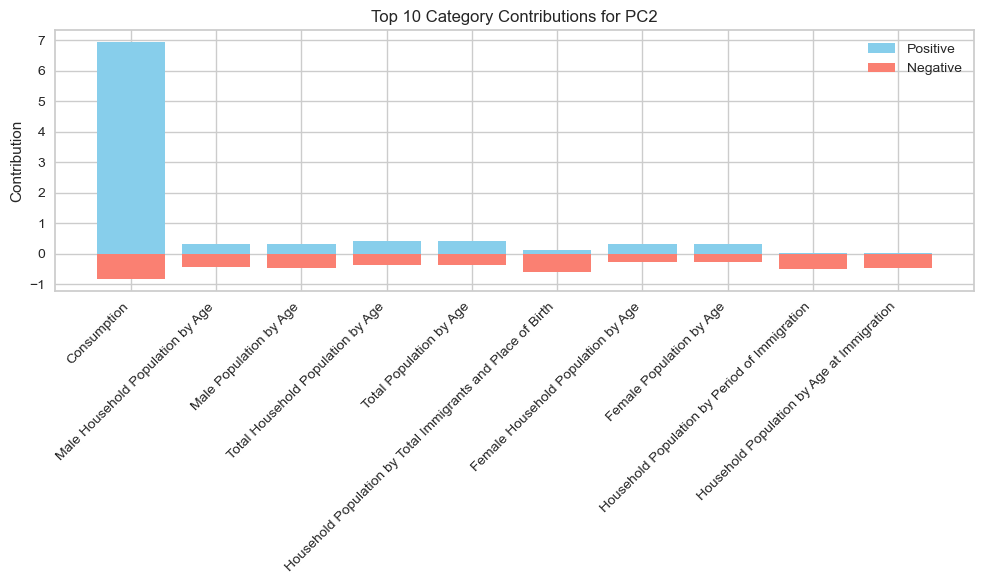
\includegraphics[width=0.75\textwidth]{figures/pc2_contribs.png}
    \caption{Top Contributing Categories to PC2}
    \label{fig:pc2}
\end{figure}

\paragraph{PC3: Household Composition and Structural Living.}  
PC3 seems to reflect differences in household structure and housing type (Figure~\ref{fig:pc3}). Contributions are more muted from \textit{Consumption}, while categories like \textit{Census Family Households by Family Structure}, \textit{Households by Household Type}, and \textit{Occupied Private Dwellings by Structure Type} contribute negatively. This suggests that lower PC3 scores may represent non-traditional or smaller households in denser housing (e.g., apartments), whereas higher scores point to more traditional family units in larger dwellings.

\begin{figure}[H]
    \centering
    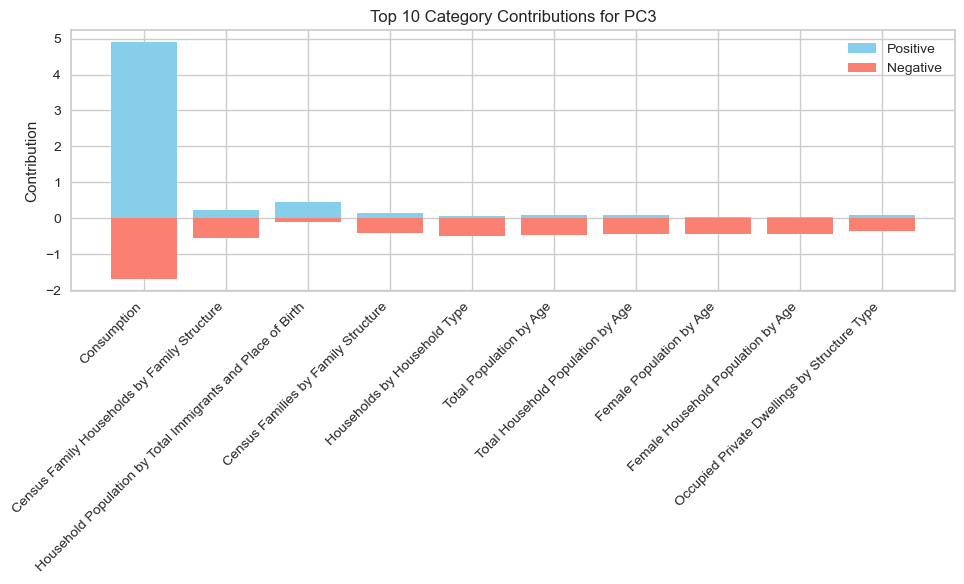
\includegraphics[width=0.76\textwidth]{figures/pc3_contribs.png}
    \caption{Top Contributing Categories to PC3}
    \label{fig:pc3}
\end{figure}

Overall, PCA revealed interpretable latent axes in the data related to economic activity, immigration patterns, and household structure. While clusters in the PCA-projected space are not strongly separable, the broad grouping captured by K-Means aligns with meaningful socioeconomic dimensions.

\paragraph{Cluster Profiling Based on Principal Components}

To better understand the characteristics of the clusters formed by K-Means ($k=3$), we calculated the average values of the first three principal components within each cluster. Since PC1 explains a dominant 67.9\% of the total variance, it serves as the primary basis for interpretation, while PC2 and PC3 (explaining 3.7\% and 3.0\%, respectively) provide additional nuance.

\begin{table}[H]
    \centering
    \caption{Mean Principal Component Scores by Cluster}
    \label{tab:cluster-pc-means}
    \begin{tabular}{@{}cccc@{}}
        \toprule
        Cluster & PC1 Mean & PC2 Mean & PC3 Mean \\
        \midrule
        0 & 37.89 & -0.63 & 0.19 \\
        1 & -15.13 & -0.22 & $\sim$0.00 \\
        2 & 5.19 & 0.80 & -0.11 \\
        \bottomrule
    \end{tabular}
\end{table}

\textbf{Cluster 0: Affluent, Traditional Immigrant Families.}  
This cluster scores highest on PC1, indicating strong consumer activity and dense, demographically diverse households. The slightly negative PC2 score suggests a moderate immigrant presence, while a mildly positive PC3 implies more traditional household structures. These could be higher-income, family-oriented areas with a mix of native and immigrant populations.

\textbf{Cluster 1: Low-Spending, High-Immigration, Small Households.}  
Cluster 1 shows the lowest PC1 score, reflecting low household spending and smaller population centers. A modestly negative PC2 indicates relatively recent immigrant populations, and the near-zero PC3 score hints at non-traditional or smaller households. These may represent younger, immigrant-dominated areas with limited consumer capacity and less conventional living arrangements.

\textbf{Cluster 2: Mid-Spending, Native, Non-Traditional Households.}  
This group is moderate on PC1 (spending) and somewhat positive on PC2, suggesting a primarily native-born population. The slightly negative PC3 implies more non-traditional household setups, such as single-person or young professional units, possibly in urban or high-density housing contexts. These areas may be characterized by moderate economic activity and non-family household compositions.

These labels will be used in subsequent visualizations and interpretation.

\subsection{Uniform Manifold Approximation and Projection}

To further investigate latent structure, we applied UMAP to reduce the high-dimensional data to two dimensions for visualization. UMAP is a non-linear technique well-suited for preserving both local and global structure in complex datasets.

We conducted a grid search over key hyperparameters: \texttt{n\_neighbors}, \texttt{min\_dist}, and \texttt{spread}, using a low \texttt{n\_epochs} of 100 for faster iteration. Three distance metrics (Euclidean, Manhattan, Cosine) were compared. Across all metrics and settings (Figures~\ref{fig:umap}, \ref{fig:umap1}, \ref{fig:umap2}), Euclidean consistently yielded the most interpretable clusters.

The best configuration was found to be \texttt{n\_neighbors=40}, \texttt{min\_dist=1}, and \texttt{spread=1.5} using the Manhattan distance metric. This setup produced compact, well-separated clusters while maintaining a balance between local cohesion and global structure.

We then re-ran UMAP with this configuration and increased \texttt{n\_epochs} to 1000 for improved convergence. The final embedding (Figure~\ref{fig:umap_final}) revealed sharper boundaries between clusters and uncovered two additional tightly packed groups not visible in PCA. These distinct clusters suggest UMAP was able to capture non-linear structures missed by PCA, reinforcing its value for exploratory analysis.

\begin{figure}[H]
    \centering
    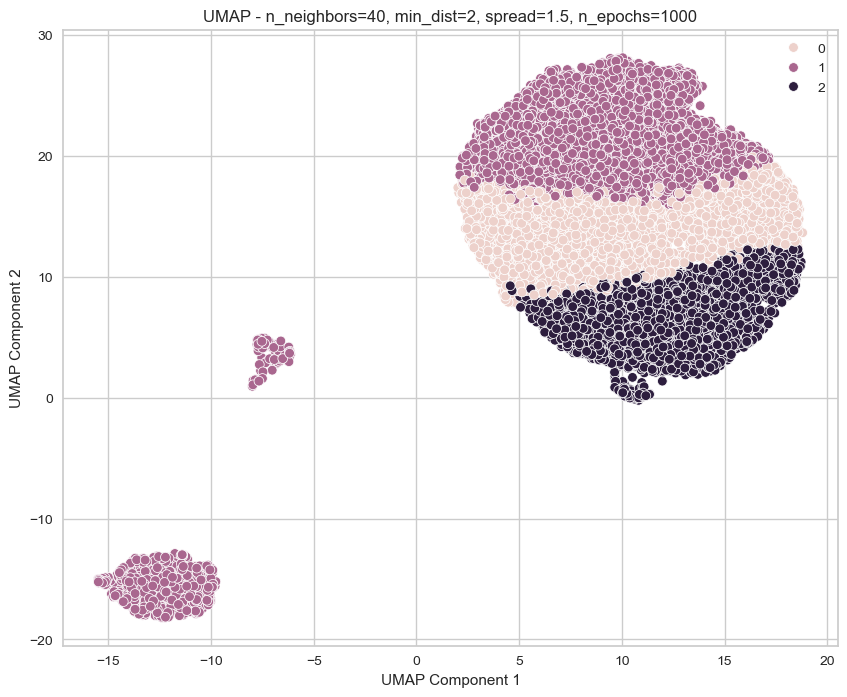
\includegraphics[width=0.7\textwidth]{figures/output3.png}
    \caption{UMAP with Manhattan distance, \texttt{n\_neighbors=40}, \texttt{min\_dist=1}, \texttt{spread=1.5}, and 1000 epochs.}
    \label{fig:umap_final}
\end{figure}


\section{Regression}
\subsection*{Target Definition \& Feature Engineering}
We define the target variable as the proportion of household income spent on personal insurance premiums and retirement/pension contributions. Concretely, if $I$ denotes total insurance spending, $P$ denotes pension contributions, and $H$ denotes household income, then
\[
  y = \frac{I + P}{H}.
\]
To prepare the data, we:
\begin{itemize}
  \item Imputed missing values using column medians.
  \item Excluded 47 columns containing keywords (``income'', ``retirement'', ``pension'', ``income tax'', ``insurance'') to avoid leakage.
  \item Dropped $\sim$300 near-constant features (low variance).
  \item Applied IQR-based winsorization to continuous predictors only, capping values at the 1.5\(\times\)IQR bounds to mitigate the influence of extreme outliers.
\end{itemize}

We retained zero–contribution cases to capture non-working households. Using correlation heatmaps, we created interaction terms (e.g., household size × insurance spending). Continuous features were winsorized at 1.5×IQR and standardized, and multi-level categoricals were one-hot encoded. This pipeline prepared the data for both linear and non-linear models.

\subsection{Elastic Net Regression}
An \texttt{ElasticNetCV} model was fit using a grid over regularization strength $\alpha \in\{0.01,0.05,0.1\}$ and mixing parameter $\ell_1$ ratio $\in\{0.1,0.3,0.5\}$, with three-fold CV and up to 10{,}000 iterations for convergence. On the test set, the model achieved
\begin{align*}
  \mathrm{MSE} &= 0.1966, \quad 95\%\,\mathrm{CI}\,[0.1948,0.1983], \\
  R^2 &= 0.8040, \quad 95\%\,\mathrm{CI}\,[0.8020,0.8058].
\end{align*}

\begin{figure}[ht]
  \centering
  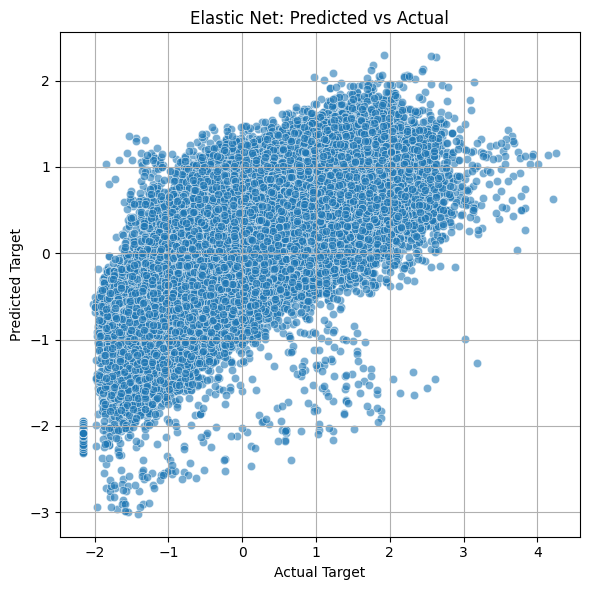
\includegraphics[width=0.75\linewidth]{figures/elastic_net_scatter.png}
  \caption{Elastic Net: Predicted vs. Actual Proportion on Test Set.}
  \label{fig:en_scatter}
\end{figure}

The top five coefficients (by magnitude) are shown in Table~\ref{tab:en_coefs}.
\begin{table}[ht]
  \centering
  \begin{tabular}{lrrp{5cm}}
    \toprule
    Feature & Coefficient & Interpretation \\
    \midrule
    ECYACTER     & +0.606 & Employment rate increases spending ratio \\
    ECYACTUR     & +0.398 & Unemployment rate increases proportion \\
    ECYMTNMED    & $-$0.224 & Higher median age reduces ratio \\
    ECYMTNAVG    & $-$0.206 & Higher average maintainer age reduces ratio \\
    HSME001S     & +0.174 & Miscellaneous spending increases ratio \\
    \bottomrule
  \end{tabular}
  \caption{Top five Elastic Net coefficients.}
  \label{tab:en_coefs}
\end{table}

We observed that $\alpha=0.01$ and $\ell_1$ ratio=0.3 were consistently selected, balancing sparsity and shrinkage. The model converged in under 2,500 iterations. All VIF scores were below 5, and residuals showed homoscedasticity and near-normality. Coefficient paths against $\alpha$ confirmed that uninformative features were quickly shrunk to zero, demonstrating effective regularization.

\subsection{XGBoost Regression}
We trained an XGBoost model using \texttt{GridSearchCV} (3-fold) over learning rate $\in\{0.05,0.1,0.2\}$, max depth $\in\{3,5,7\}$, and n\_estimators $\in\{100,200,300\}$. The optimal parameters were
\[
  \text{learning\_rate}=0.1,
  \quad \text{max\_depth}=5,
  \quad n\_\mathrm{estimators}=200.
\]
Test performance improved substantially:
\begin{align*}
  \mathrm{MSE} &\approx 0.0888, \quad 95\%\,\mathrm{CI}[0.0880,0.0896], \\
  R^2 &\approx 0.9114, \quad 95\%\,\mathrm{CI}[0.9105,0.9123].
\end{align*}

\begin{figure}[ht]
  \centering
  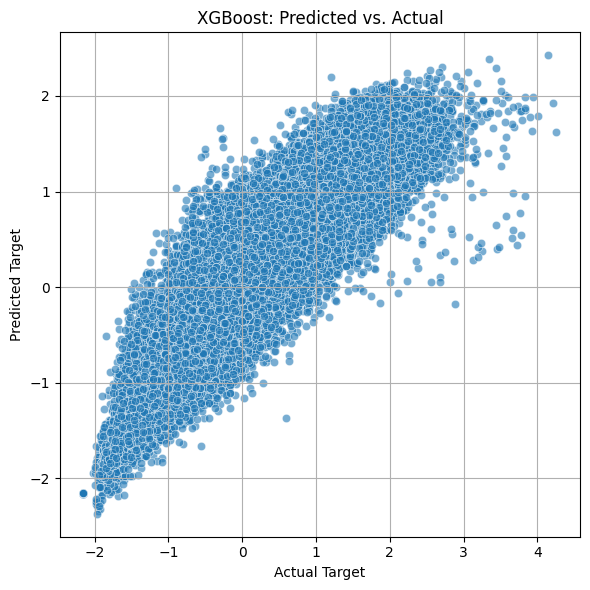
\includegraphics[width=0.75\linewidth]{figures/xgb_scatter.png}
  \caption{XGBoost: Predicted vs. Actual Proportion on Test Set.}
  \label{fig:xgb_scatter}
\end{figure}

We used early stopping (50 rounds) to prevent overfitting. Feature importance (gain and cover) matched SHAP rankings. Partial dependence plots for \texttt{HSHO002} and \texttt{ECYMTNMED} showed non-linear threshold effects. Sensitivity tests confirmed that \texttt{max\_depth}=5 balanced interaction capture and variance. These findings highlight XGBoost’s ability to model complex patterns beyond linear methods.

\subsection{SHAP-Based Interpretation}
We computed SHAP values on the test set to quantify feature contributions. Table~\ref{tab:shap_top5} shows the top five features by mean $\left|\text{SHAP}\right|$, and Figure~\ref{fig:shap_hsho002} displays the dependence plot for \texttt{HSHO002}.

\begin{table}[ht]
  \centering
  \caption{Top five features by mean |SHAP| (XGBoost)}
  \begin{tabular}{llr}
    \toprule
    \textbf{Feature} & \textbf{Description}                       & $\mathbf{\overline{\lvert\text{SHAP}\rvert}}$ \\
    \midrule
    HSHO002  & Number of housekeepers employed            & 0.137 \\
    HSSH042  & Mortgage on secondary residences           & 0.129 \\
    HSMG001S & Total money gifts and contributions        & 0.125 \\
    ECYMTNMED& Median maintainer age                     & 0.101 \\
    HSCC002  & Childcare outside the home                 & 0.083 \\
    \bottomrule
  \end{tabular}
  \label{tab:shap_top5}
\end{table}

\begin{figure}[ht]
  \centering
  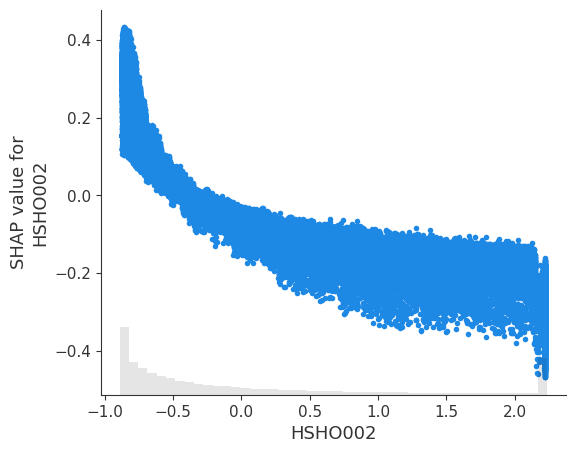
\includegraphics[width=0.75\linewidth]{figures/shap_dependence_hsho002.png}
  \caption{SHAP dependence plot for \texttt{HSHO002}.}
  \label{fig:shap_hsho002}
\end{figure}

For each of the top five features, key SHAP-based behaviors include:
\begin{itemize}
  \item \textbf{HSHO002}: Values below approximately two housekeepers drive strong positive contributions, while higher counts reverse to negative impacts, indicating threshold-like effects (Fig.~\ref{fig:shap_hsho002}).
  \item \textbf{HSSH042}: Negative contributions intensify for large secondary mortgage values, consistent with heightened budget constraints under elevated debt loads.
  \item \textbf{HSMG001S}: Small to moderate gift and contribution amounts yield positive effects, but marginal impact diminishes at higher values, suggesting diminishing returns.
  \item \textbf{ECYMTNMED}: Consistently negative impact on predicted spending, with a sharper decline at extreme ages, highlighting accelerated non-linear aging effects.
  \item \textbf{HSCC002}: Low levels of childcare outside the home contribute positively and steeply, then plateau, reflecting interplay with total household support expenditures.
\end{itemize}

We used SHAP interaction values to detect pairwise effects, notably between \texttt{HSHO002} and \texttt{HSCC002}. Individual explanations showed how feature contributions sum to predictions. A summary dot plot (not shown) revealed variability for extreme \texttt{HSMG001S} values. However, correlated features can share attribution. Overall, SHAP provides reliable global and local insights for policy decisions.

\subsection*{Conclusions and Recommendations}

We predicted insurance and pension spending accurately with both methods. Elastic Net ($R^2=0.8040$) highlighted key macroeconomic and demographic drivers. XGBoost ($R^2\approx0.9114$) captured non-linear, threshold effects (e.g.\ housekeeper counts, gift contributions) that Elastic Net missed. SHAP confirmed these non-linear patterns and provided actionable global and local insights.

\begin{itemize}
  \item \textbf{Deploy the XGBoost model in production}, with routine monitoring of predictive performance and recalibration every quarter. Leverage early-stopping and validation-based retraining to guard against concept drift.
  \item \textbf{Integrate SHAP-driven alerts} into decision workflows. For example, flag households with extreme SHAP values on \texttt{HSHO002} or \texttt{HSMG001S} to target outreach or adjust product offerings.
  \item \textbf{Segment the customer base} by key drivers uncovered (e.g.\ median maintainer age, household support expenditures). Tailor marketing and education campaigns—for younger households, emphasize pension benefits; for high secondary-mortgage clients, highlight insurance products that mitigate debt risk.
  \item \textbf{Expand data coverage} to include behavioral and psychographic variables (e.g.\ online engagement, risk tolerance surveys) to refine model granularity and support personalized recommendations.
  \item \textbf{Establish a governance framework} for model explainability and fairness. Regularly audit feature importances and SHAP interactions to ensure no adverse or biased effects on underserved groups (e.g.\ unemployed or non-working-age segments).
  \item \textbf{Conduct A/B tests} to quantify the lift from model-driven interventions versus standard strategies, using metrics such as contribution rate uplift and retention.
\end{itemize}

\appendix
\section*{Appendix}

\section{Experiment Notebooks}
The Jupyter Notebooks in which our experiments and analysis were conducted are provided alongside this report. The work related to Clustering and Principal Component Analysis can be found in \texttt{Clustering\_and\_PCA.ipynb}. UMAP related works are provided in \texttt{UMAP.ipynb}, and all regression related work is in \texttt{Part\_2.ipynb}.

\section{Extra Silhouette Plots}

\begin{figure}[H]
    \centering
    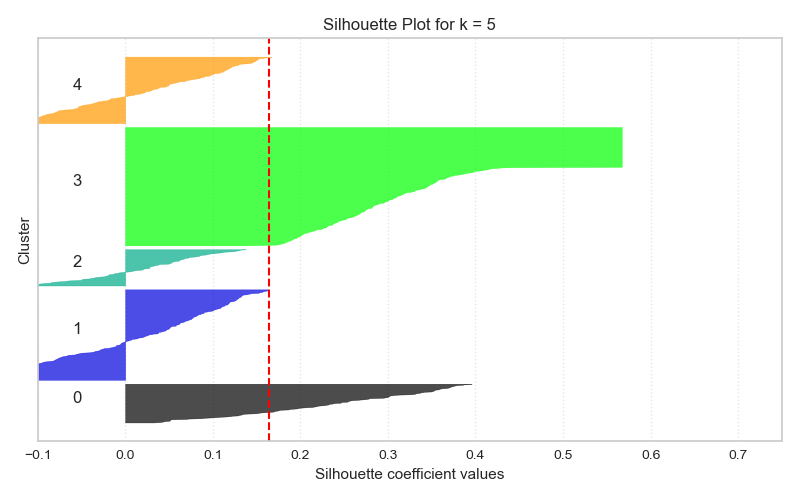
\includegraphics[width=0.6\textwidth]{figures/silhouette_k5.png}
    \caption{Silhouette Plot for $k=5$}
    \label{fig:silhouette_k5}
\end{figure}

\begin{figure}[H]
    \centering
    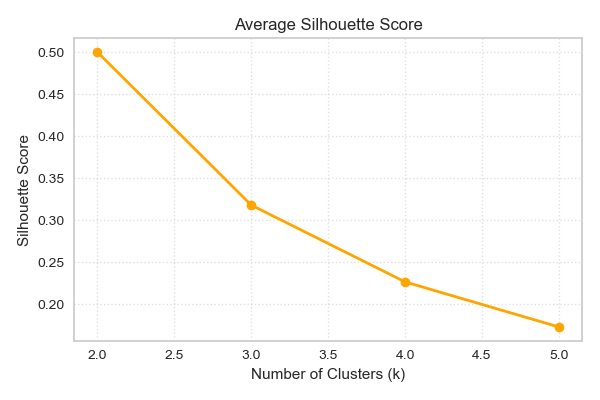
\includegraphics[width=0.65\textwidth]{figures/silhouette_scores.png}
    \caption{Average Silhouette Scores for $k=2$ to $k=5$}
    \label{fig:silhouette_scores}
\end{figure}


\section{PCA Component Loadings}

The following tables show the top five positive and negative variable loadings for each of the first three principal components (PC1–PC3). These values were used to interpret the latent dimensions of the PCA results. HHS refers to the HouseholdSpend dataset.

\begin{table}[H]
\centering
\caption{Top Positive Loadings for PC1}
\label{tab:pc1_pos}
\begin{tabular}{@{}lllll@{}}
\toprule
Variable & HHS Description & HHS Type & DemoStats Category & Loading \\
\midrule
ECYHOMSING & - & - & Language Spoken Most Often At Home & 0.04791 \\
ECYMOTSING & - & - & Mother Tongue & 0.04789 \\
ECYMOBHPOP & - & - & 5-Year Mobility & 0.04789 \\
ECYAIDHPOP & - & - & Indigenous Identity & 0.04788 \\
ECYRIMHPOP & - & - & Recent Immigrants (2017–Present) & 0.04788 \\
\bottomrule
\end{tabular}
\end{table}

\begin{table}[H]
\centering
\caption{Top Negative Loadings for PC1}
\label{tab:pc1_neg}
\begin{tabular}{@{}lllll@{}}
\toprule
Variable & HHS Description & HHS Type & DemoStats Category & Loading \\
\midrule
ECYMTNMED & - & - & Maintainer Age & -0.00437 \\
ECYPFAMED & - & - & Female Population by Age & -0.00413 \\
ECYHFAMED & - & - & Female Household Population by Age & -0.00348 \\
ECYPMAMED & - & - & Male Population by Age & -0.00348 \\
ECYHMAMED & - & - & Male Household Population by Age & -0.00282 \\
\bottomrule
\end{tabular}
\end{table}

\begin{table}[H]
\centering
\caption{Top Positive Loadings for PC2}
\label{tab:pc2_pos}
\begin{tabular}{@{}lllll@{}}
\toprule
Variable & HHS Description & HHS Type & DemoStats Category & Loading \\
\midrule
HSSH037A & Wood/Fuel for Heating & Consumption & - & 0.11518 \\
ECYHTAMED & - & - & Household Pop. by Age & 0.11505 \\
ECYPTAMED & - & - & Total Population by Age & 0.11242 \\
ECYHMAMED & - & - & Male Household Population by Age & 0.10444 \\
HSSH034 & Other Fuel & Consumption & - & 0.10254 \\
\bottomrule
\end{tabular}
\end{table}

\begin{table}[H]
\centering
\caption{Top Negative Loadings for PC2}
\label{tab:pc2_neg}
\begin{tabular}{@{}lllll@{}}
\toprule
Variable & HHS Description & HHS Type & DemoStats Category & Loading \\
\midrule
ECYNCA\_18P & - & - & Citizenship & -0.09457 \\
ECYVISVM & - & - & Visible Minority Status & -0.09315 \\
ECYHOMNOFF & - & - & Language Spoken Most Often At Home & -0.09130 \\
ECYNCANCIT & - & - & Citizenship & -0.09076 \\
ECYPIM1621 & - & - & Period of Immigration & -0.08743 \\
\bottomrule
\end{tabular}
\end{table}

\begin{table}[H]
\centering
\caption{Top Positive Loadings for PC3}
\label{tab:pc3_pos}
\begin{tabular}{@{}lllll@{}}
\toprule
Variable & HHS Description & HHS Type & DemoStats Category & Loading \\
\midrule
HSWH040S & Net Purchase Price of Residences & Consumption & - & 0.13164 \\
HSTE001ZBS & Non-current Consumption & Consumption & - & 0.12020 \\
HSSH033A & Natural Gas (Owned Residence) & Consumption & - & 0.11436 \\
HSSH033 & Natural Gas & Consumption & - & 0.10837 \\
ECYCHAHHCH & - & - & Children at Home by Age & 0.10319 \\
\bottomrule
\end{tabular}
\end{table}

\begin{table}[H]
\centering
\caption{Top Negative Loadings for PC3}
\label{tab:pc3_neg}
\begin{tabular}{@{}lllll@{}}
\toprule
Variable & HHS Description & HHS Type & DemoStats Category & Loading \\
\midrule
ECYSTYAPU5 & - & - & Structure Type & -0.13074 \\
ECYMOTFREN & - & - & Mother Tongue & -0.12838 \\
ECYSTYAPT & - & - & Structure Type & -0.12515 \\
ECYHOMFREN & - & - & Language Spoken Most Often At Home & -0.12314 \\
\bottomrule
\end{tabular}
\end{table}

\section{Varying UMAP Distance Metric Plots}
\begin{figure}[H]
    \centering
    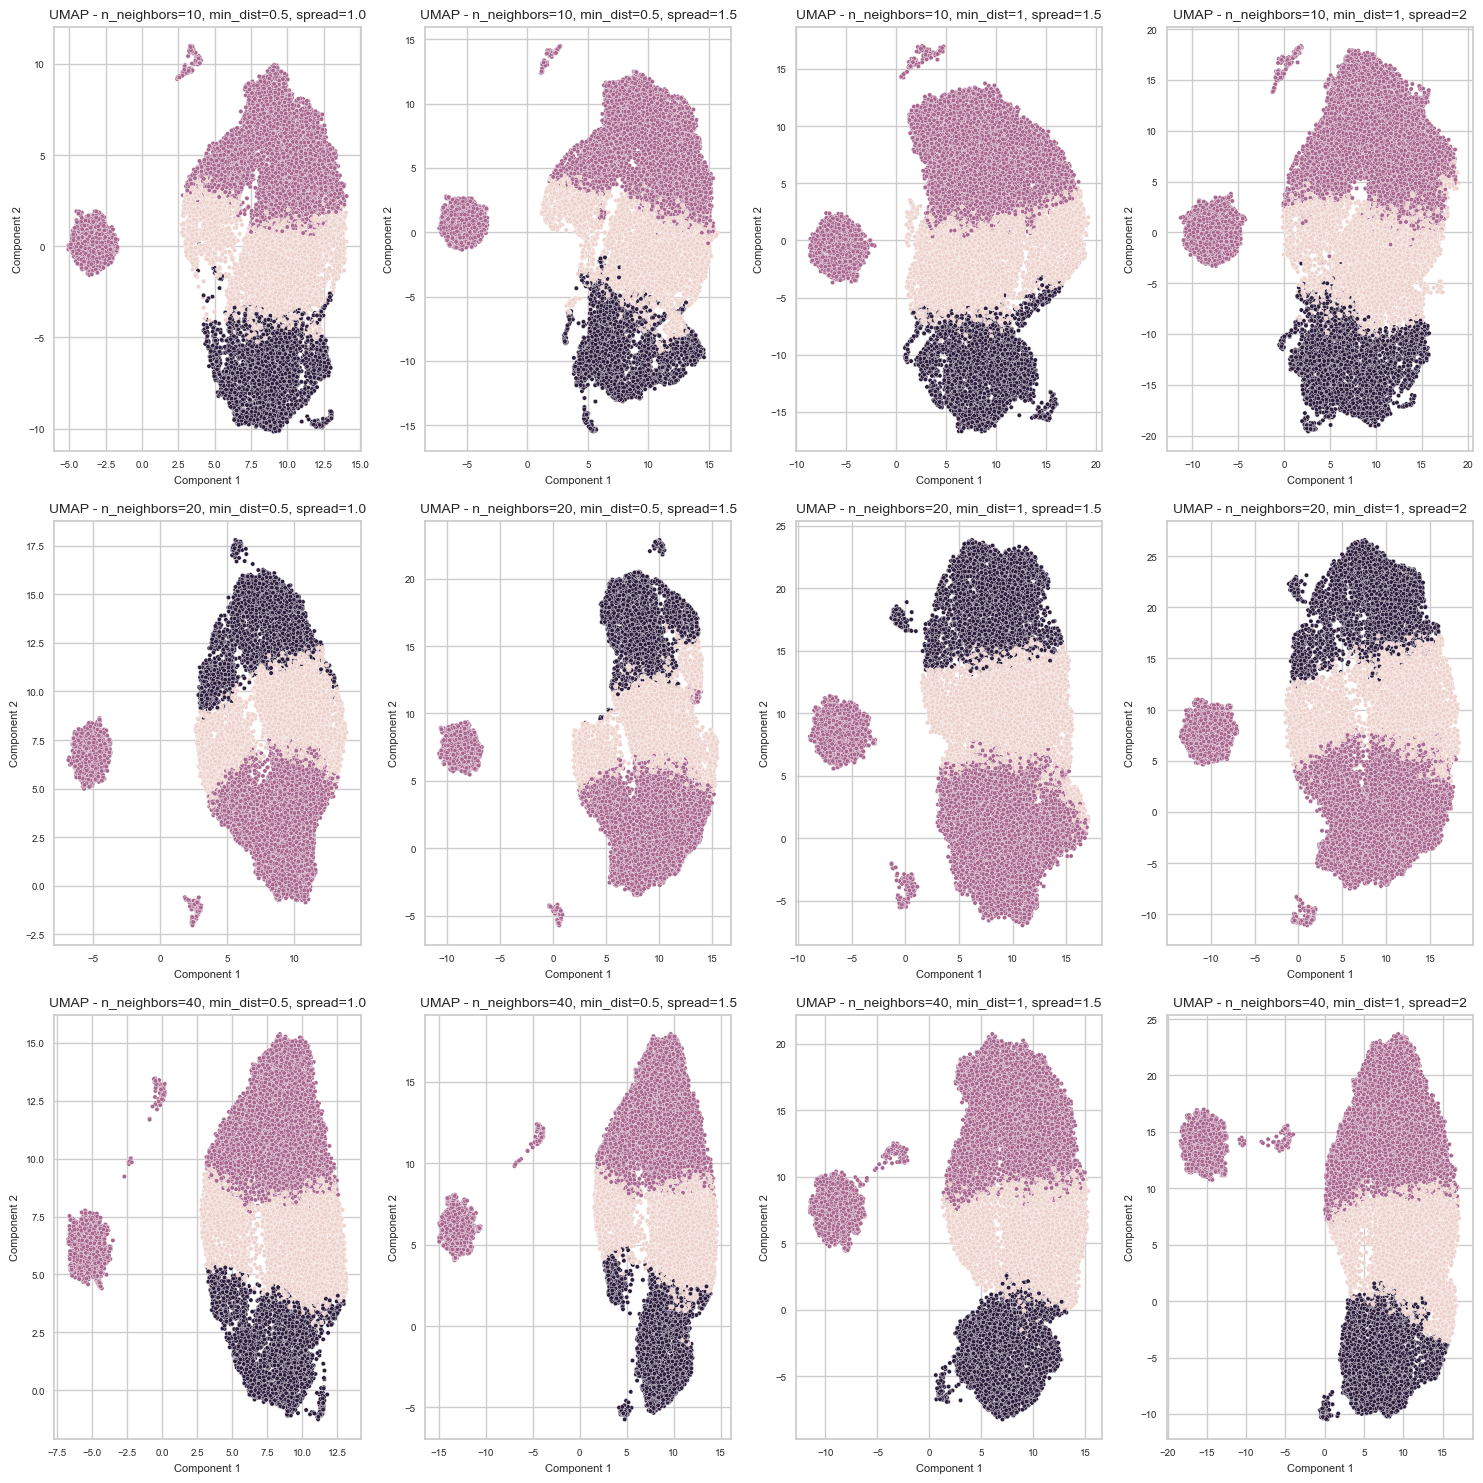
\includegraphics[width=0.8\textwidth]{figures/output.png}
    \caption{UMAP with euclidean distance metric and different values of n\_neighbors, min\_dist and spread.}
    \label{fig:umap}
\end{figure}
\begin{figure}[H]
    \centering
    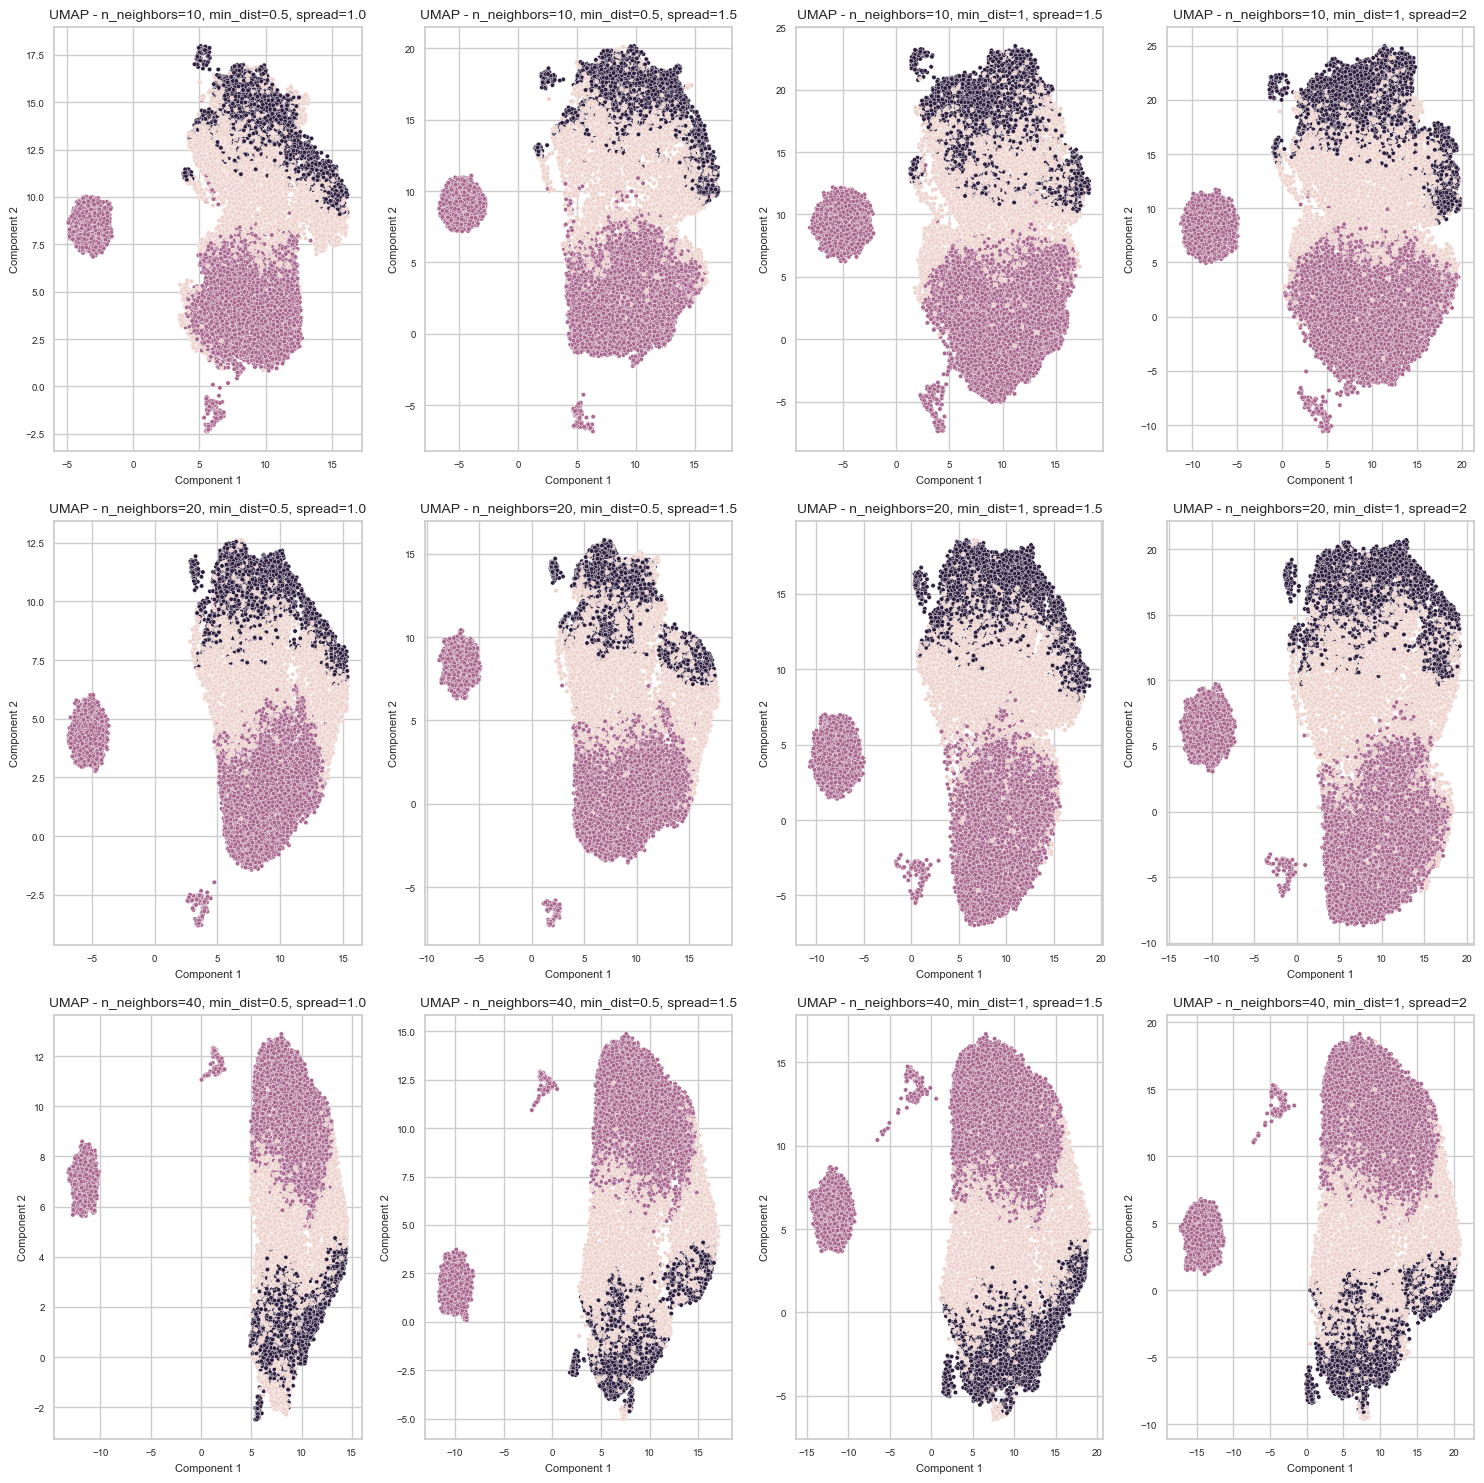
\includegraphics[width=0.8\textwidth]{figures/output1.png}
    \caption{UMAP with cosine distance metric and different values of n\_neighbors, min\_dist and spread.}
    \label{fig:umap1}
\end{figure}
\begin{figure}[H]
    \centering
    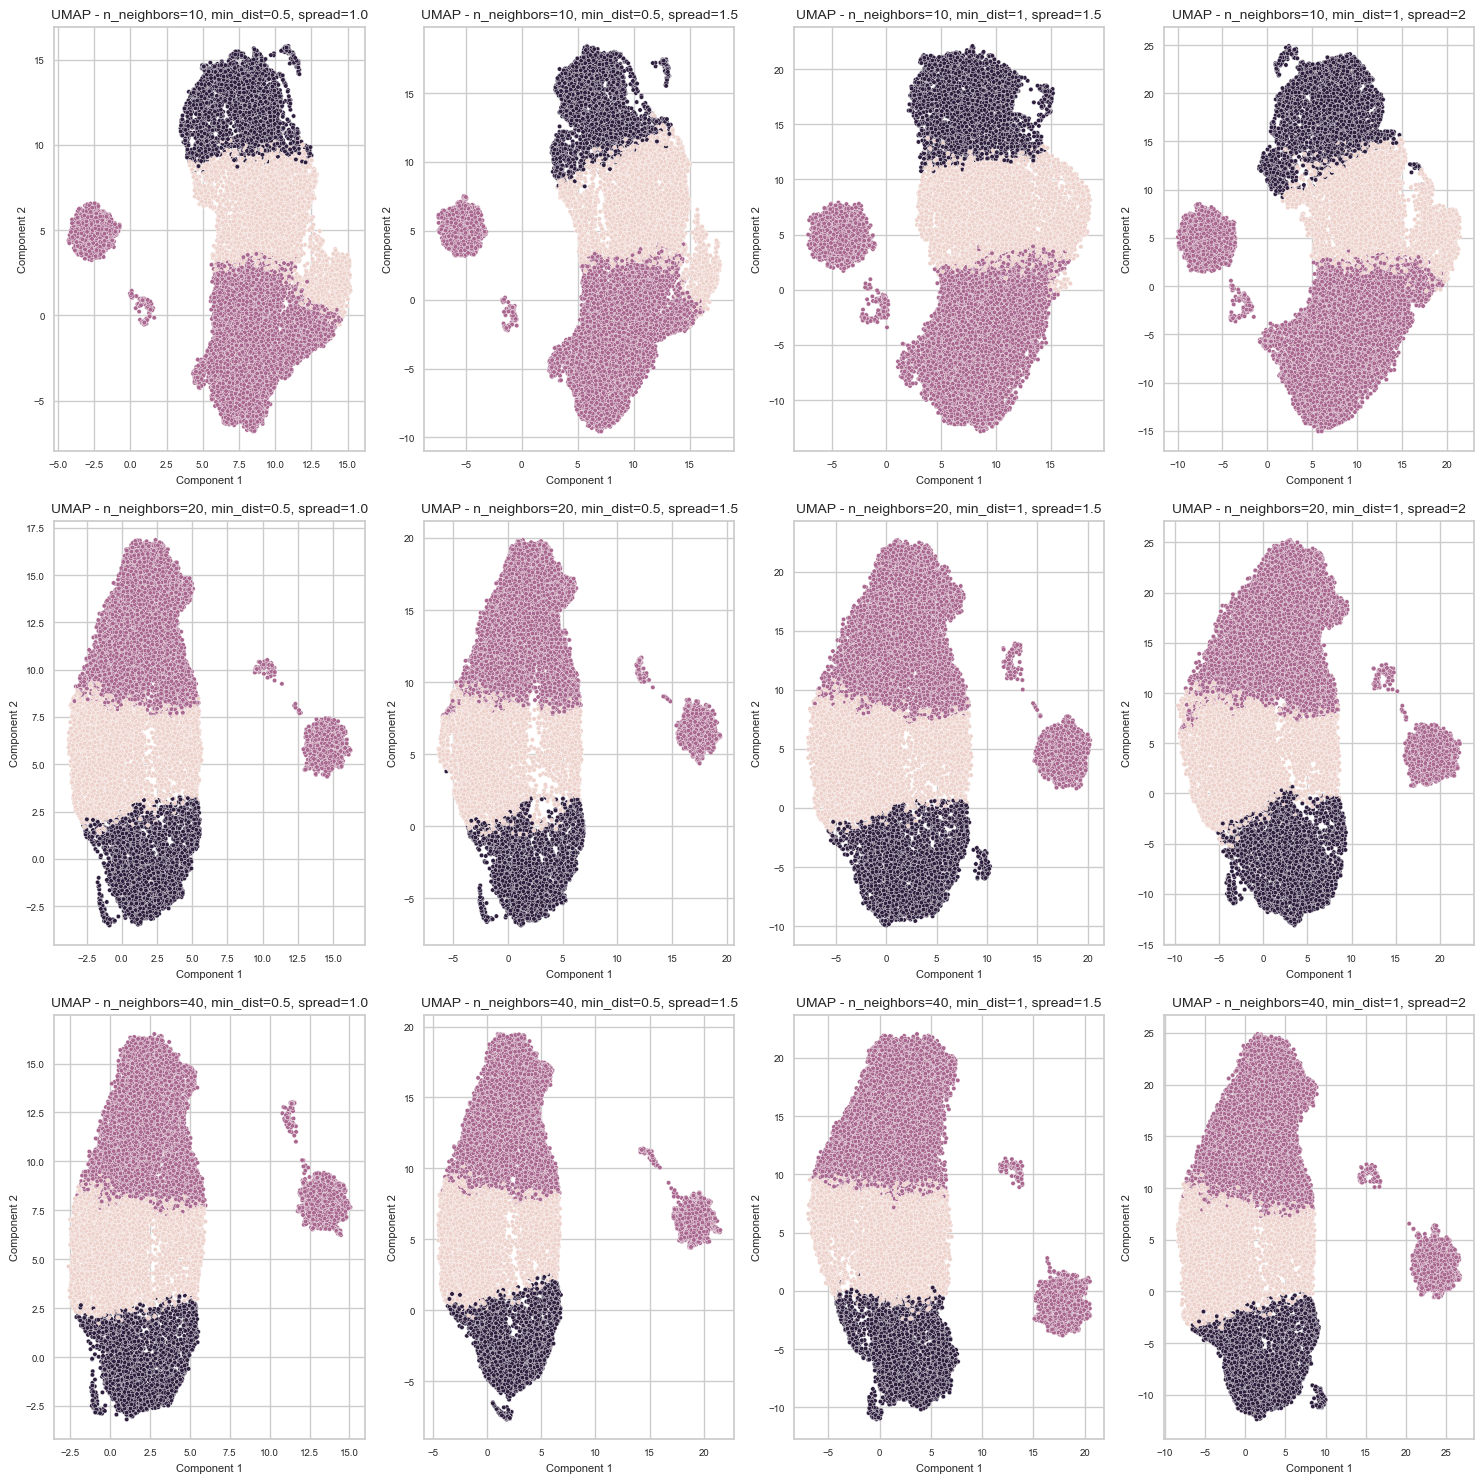
\includegraphics[width=0.8\textwidth]{figures/output2.png}
    \caption{UMAP with manhattan distance metric and different values of n\_neighbors, min\_dist and spread.}
    \label{fig:umap2}
\end{figure}

\section{SHAP Plots for Additional Variables}

\begin{figure}[H]
  \centering
  \begin{subfigure}{0.45\textwidth}
    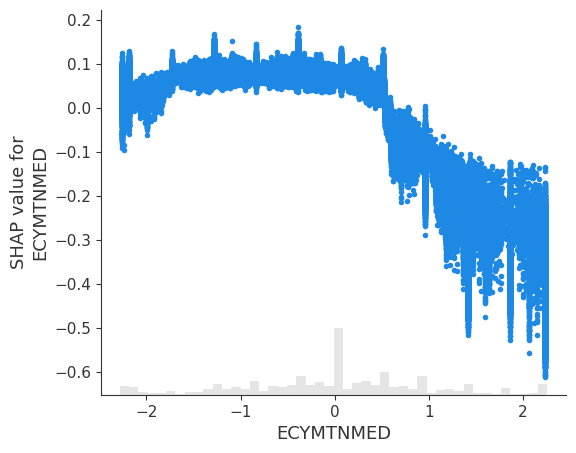
\includegraphics[width=\linewidth]{figures/ECYMTNMED_SHAP.png}
    \caption{SHAP for ECYMTNMED}
  \end{subfigure}
  \hfill
  \begin{subfigure}{0.45\textwidth}
    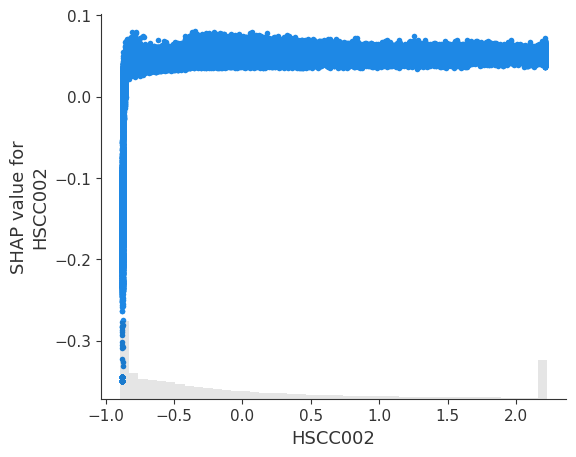
\includegraphics[width=\linewidth]{figures/HSCC002_SHAP.png}
    \caption{SHAP for HSCC002}
  \end{subfigure}

  \vspace{0.5cm}

  \begin{subfigure}{0.45\textwidth}
    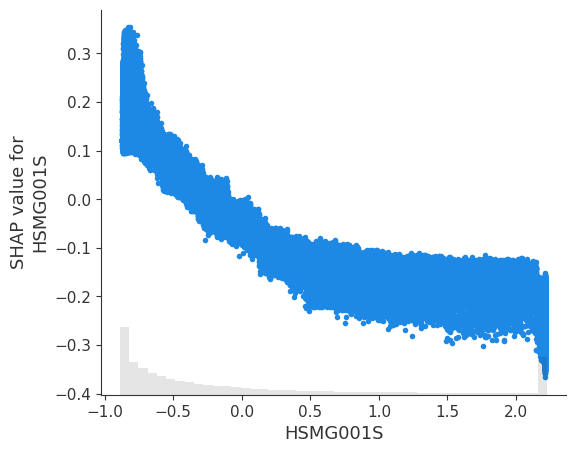
\includegraphics[width=\linewidth]{figures/HSMG001S_SHAP.png}
    \caption{SHAP for HSMG001S}
  \end{subfigure}
  \hfill
  \begin{subfigure}{0.45\textwidth}
    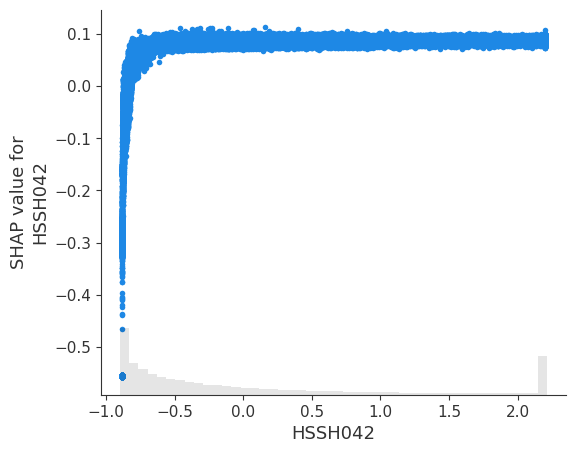
\includegraphics[width=\linewidth]{figures/HSSH042_SHAP.png}
    \caption{SHAP for HSSH042}
  \end{subfigure}
  
  \caption{SHAP Value Graphs for Additional Variables}
\end{figure}


\end{document}